\chapter{General Conclusions}
\label{chapterlabel6}
In this chapter we will conclude this thesis by first summarising the impact of the optimisation changes made to \textbf{Contur} as part of this research project. We will then finish up by highlighting the remaining parts of \textbf{Contur} that could potentially be further optimised in the future.

\section{Results Summary}

In figure \ref{fig:final_grid_profile} below we can see the final profile of the grid run, comparing to figure \ref{fig:grid_yoda_start_profile} which shows the initial profile of the grid run before any optimisation, we can see the full impact of the changes made as part of this research project. From a starting runtime of close to 20 minutes before optimisation, the changes made as part of this project have taken the runtime below 4 minutes. The optimisation of the likelihood calculation outlined in section \ref{sec:likelihood} is the largest contributor to this runtime reduction. The change to the \texttt{sort\_blocks()} method outlined in section \ref{sortBlocksSection} was also a material contributor to the runtime reduction.

\begin{figure}[H]
\centering
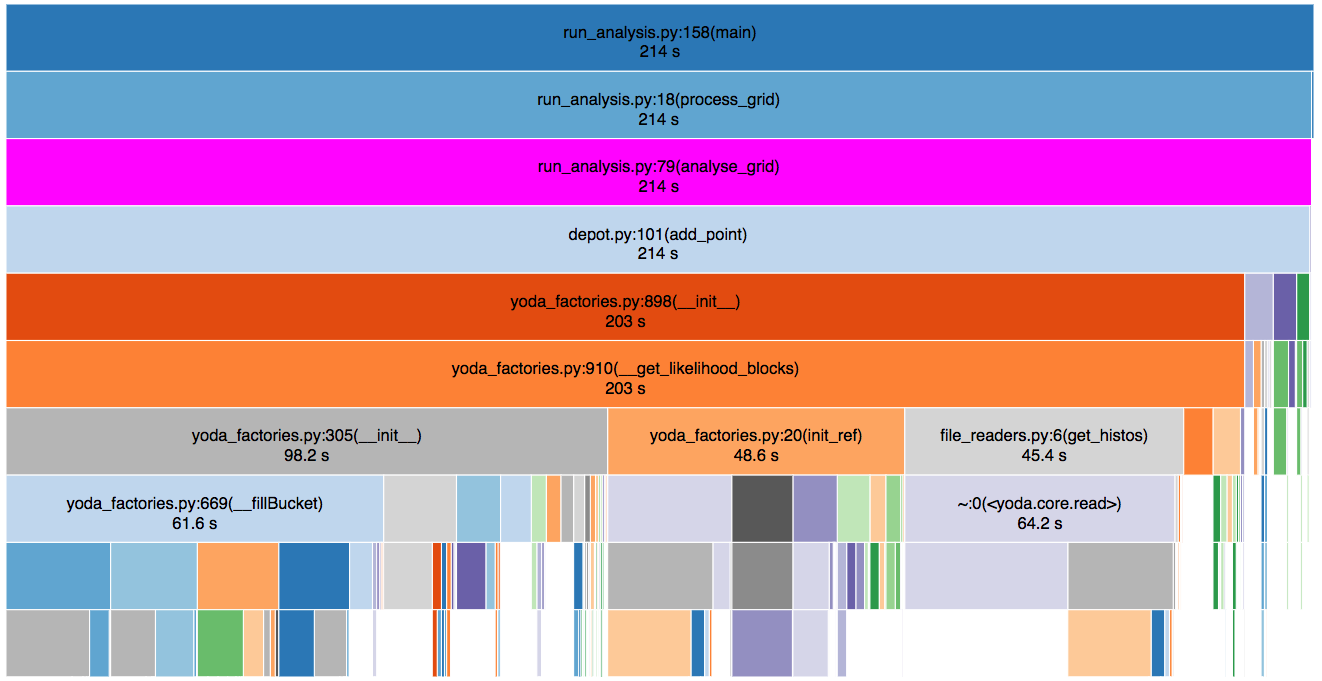
\includegraphics[scale=0.3]{plots/final_grid_profile.png}
\caption{Final Grid Profile}
\label{fig:final_grid_profile}
\end{figure}

\section{Future Work}
The profiling results in figure \ref{fig:final_grid_profile} above can also be examined to understand the areas of \textbf{Contur} that now occupy the most runtime after the optimisations implemented in this research project. From the figure we can identify three main blocks of runtime, one from the initialisation of \classname{yoda\_factories}, another from the \texttt{init\_ref()} method and the final piece from the \texttt{get\_histos()} method.

The \texttt{init\_ref()} and \texttt{get\_histos()} methods are mainly preoccupied with reading \textbf{YODA} files into \textbf{Contur}. So after our optimisation we can say that nearly half of \textbf{Contur's} runtime comes from reading \textbf{YODA} files. This is not something that can be further optimised in \textbf{Contur} in isolation, instead further optimisations can only be achieved here via making the reading of \textbf{YODA} files faster. So this is an optimisation that would likely have to take place within the \textbf{YODA} package.

In the other block of runtime coming from instantiating the \classname{yoda\_factories}, when we drill down we can also see that a lot of runtime here comes from calling \textbf{YODA} methods\footnote{The main examples are \texttt{yVals}, \texttt{yErrs} and \texttt{xErrs}, all of which are found in \texttt{yoda.core.Scatter2D}}. So the conclusion here as well is that the best means for further optimisations in \textbf{Contur} comes from optimisations in  \textbf{YODA}.
